% Architecture Description and system specifications
% 	* Multisensor IMS		
%		* Processing Stages
%		* Fusion approaches		
%	* Validation approaches
%		* Transportation and Traffic Simulations
%			* Simulators Classification
%		* Intersection monitoring Datasets
%			* POSSi Dataset
%			* KoPER Dataset
%	* Architecture proposal

\chapter [Architecture Description and System Specification]{Architecture Description and System Specification}
\chaptermark {System Description}

\epigraph{"Perfect is enemy of good"}{Voltaire}

Although several types of sensors are used for intersection monitoring and supervision, the use of cameras, lasers and lidars has increased due to advances in sensors manufacturing and computing capabilities. Such enhancements allows to deploy more of those types of sensors per scenario and it is required to define some processing stages from raw data capture through decision and control stages. It is also needed to test and validate the developments prior to a real and full functional implementation. The first part of this chapter describes the main stages in a intersection management system, from data preprocessing to situation assesment. Then, two validation tools for IMS applications are described, simulation models and datasets. And finally, the proposed architecture for the implementation of an IMS system is presented.

\section{Multisensor IMS}

Multicamera and multilasers monitoring systems offer more information about environment that can be merged to provide a better representation of the whole scene, detect with more accuracy the objects in the intersection, and prevent possible incidents. For designing a single-sensor or multi-sensor IMS, there are some basic processing stages to have into account. In the case of a multisensor system, it is also required to analyse and determine which is the better fusion approach to use and in which of the processing stages this fusion should be performed, in order to get better results than a single-sensor based system.

\subsection{Processing Stages}

%\todo{Check stages description and figure}

In the designing of an IMS, there are four main stages that have to be performed from the data source to final output: preprocessing, feature analysis, pattern recognition and situation assessment. The aim of the first stage is to extract data of interest from the raw sensor information, using filtering to remove noise and irrelevant data, and background subtraction techniques to get the foreground of the scene. Spatial-temporal alignment of data is also performed in this stage. In the second stage, the objective is to identify elements within the foreground and extract relevant features of them. The third stage receives the set of features from the previous stage and performs recognition and classification tasks. Also, tracking and prediction of objects' state is performed based on historic information. In the fourth stage, object behaviour and inter-objects interaction are analysed to identify context and detect situations or events of interest. This output could be delivered to an automated or semi-automated stage of decision and control, to a human operator, or to a traffic agent or institution, to take immediate actions on traffic control, issue traffic tickets, warn drivers about possible incidents or improve transportation policies in a long-term basis. In figure \ref{proc_stages}, previously described stages are depicted, including a list of common tasks performed at each of these stages.

\begin{figure}[ht!]
\centering
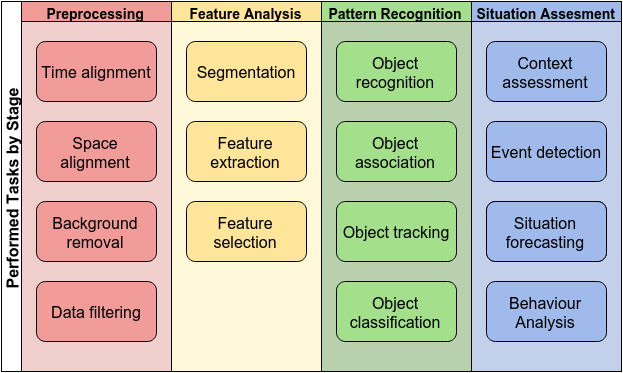
\includegraphics[scale=0.55]{fig/3/processing_stages_and_tasks.png}
\caption{Processing stages in an IMS and commonly performed tasks within each of them}
\label{proc_stages}
\end{figure}


\subsection{Fusion approaches}

Depending on wheter the system has multiple sensors of the same type or different type, a data fusion approach should be chosen. When data came from same-type sensors, it is usually fused at low levels using techniques for temporal-spatial alignment, depending on sensors configuration. This is the case for a network of lasers or lidars or for multi-camera systems. If the system have different type of sensors, data from them may be fused at mid level, based on extracted features or classes on each subsystem; or may be fused at high level if each subsystem delivers control or decision outputs. The tasks shown in each of the processing stages (Figure \ref{proc_stages}), could be used as fusion blocks for homogeneous or heterogeneous data.

\section{Validation approaches}

Before deploying an IMS, it is needed to test some of its components and validate their results. Two commonly used tools for this purpose are traffic simulation models and datasets, depending on the component to be tested. Below, a description of each one is presented.

\subsection{Transportation and Traffic Simulation}

Transportation is a highly complex activity where different elements, like infrastructure, vehicles and pedestrians, affect efficiency, safety and quality of traffic. Intersections are special cases because there exists a high interaction between those mentioned elements making of these places critical points for mobility. For this reason, it is needed to have traffic models to allow the simulation of new policies or deployments intended to enhance transportation.

Three widely-known models for this kind of analysis are macroscopic model, microscopic model and mesoscopic model. The macroscopic model of traffic flow is based on a hydrodynamic analogy, modeling traffic as a fluid process characterized by three main variables, density, volume and speed, and the objective is to describe time-space evolution of those variables. The microscopic model aims to detail at a high detail inter-vehicles interactions and their individual state. For example, in a lane-change maneuver the state of the car doing the action and those affected by it, is individually tracked. The mesoscopic model tries to include features of both macroscopic and mesoscopic model. In this case, the same lane-change maneuver could be seen as an instant action triggered by lane density rather than on individual interactions.

%\todo{Simulators description (?)}

A more detailed analysis of traffic simulation models and simulation platforms could be found in \cite{AdamsBoxill2000, Barcelo2000, Kitamura2005, Lieberman1992}




\subsection{Intersection monitoring Datasets} \label{possi_ds}

As mentioned in section \ref{s23}, POSS-i \footnote{Available at http://www.poss.pku.edu.cn/download.html} and Ko-PER \footnote{Available at http://www.uni-ulm.de/in/mrm/forschung/datensaetze.html} projects are leading the development of multisensor Intersection Management Systems. One of the contributions of these projects is the creation of datasets of such systems. They provide camera and laser information of a monitored intersection in Peking, China and Aschaffenburg, Germany, respectively.

%Next, a description of these two datasets will be given.
%
%\subsubsection{POSSi Dataset } \label{possi_ds}
%
%POSSi dataset\footnote{Available at http://www.poss.pku.edu.cn/download.html}
%
%\todo{Dataset description (?)}
%
%\subsubsection{KoPER Dataset }
%
%Ko-PER dataset\footnote{Available at http://www.uni-ulm.de/in/mrm/forschung/datensaetze.html}
%
%The full description of this dataset is presented in \cite{Strigel2014}.

\section{Architecture proposal}

The proposal presented in this work is based on MFI model processing entities in the sense that a processing block could take one or more inputs related between them and generate an output of the same type or a higher level output, that means that some blocks perform fusion while others just do some processing on incoming data. The communication or data exchange approach is based on JDL model, in which data is available over a "bus", where the processing blocks can write to or read from. And an information model is defined for abstract the elements of the scene, set a format for message exchange and define global and local configuration parameters. A general block diagram is shown in figure \ref{proposal_blocks}.

\begin{figure}[ht!]
\centering
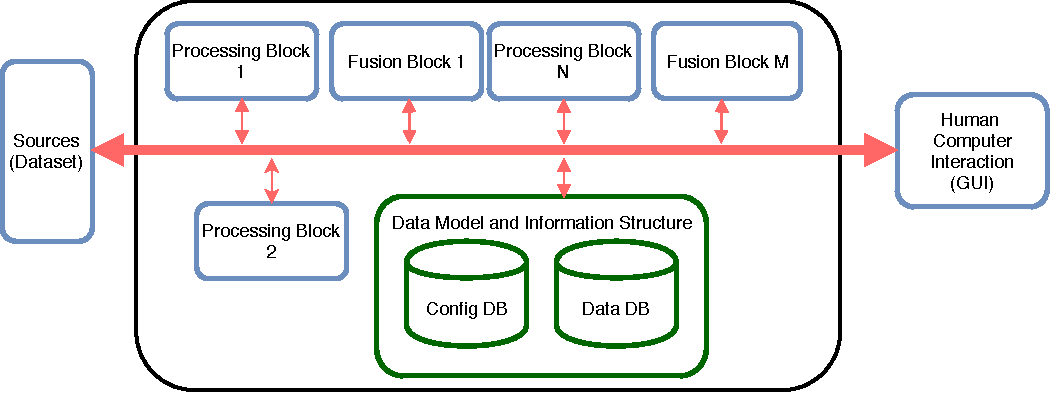
\includegraphics[scale=0.7]{fig/3/proposal_blocks.pdf}
\caption{General overview of proposed architecture and its components. Red for the communication scheme, green for data model and blue for processing blocks}
\label{proposal_blocks}
\end{figure} 

%\todo{Design Considerations}

As the implementation of a full Intersection Management System is a joint effort among different fields of engineering (Hardware, software, IT, civl) and even non-engineering areas, The two main features chosen for this proposal are scalability and modularity. Scalability is desired in the cases where an initial deployment needs to expand or increase its complexity in any of its areas, for example, new communication approaches, add new sensors or hardware, develop new features or policies, etc. Modularity allows that the internal blocks of system could be modified, exchanged or enhanced without disturbing the overall function of the deployment. This criteria is achieved with the four proposed elements of this architecture: communication scheme, data model, information structure and processing blocks. 


\subsection{Communication scheme}

In order to isolate the processing tasks of the communication system, a Publisher-Subscriber approach is selected. The benefits of this option is that data can be shared between diferent blocks without generating a dependency from publishers to subscribers. Another benefit is that exposing a defined mechanism for publishing or subscribing, allows the system to be implementation agnostic.

Taking these reasons into account, Redis is chosen as communication platform. As stated in their website, "Redis is an open source (BSD licensed), in-memory data structure store, used as a database, cache and message broker"\cite{Redis} which support Publisher-Subscriber paradigm, allowing greater scalability and a more dynamic network topology.

For publishers and subscribers to exchange messages, channels are defined with labels using a namespace approach that describe the source of data and the kind of data. For example a channel containing raw data from a laser scanner could be labeled as \texttt{/sensors/range/laser\_1/data/raw}.

Redis is also used as in-memory storage for configuration data that is not part of the processing flow, like sensor parameters, intersection model and control options. This information is loaded into Redis from a configuration file formatted using JavaScript Object Notation (JSON), and once loaded in Redis, it is available for any client requiring it.

%\todo{Define JSON HERE!!!!}

\subsection{Data Model}

The data model proposed for the system includes the abstraction of the sensing elements and the intersection model. For the sensing elements, a Sensor base class and two derived classes, RangeSensor class and ImageSensor class, are defined. 

The intersection has been modeled as a class with attributes like a label, a Map object, a set of RangeSensors and CameraSensors objects, a set of Leg objects, and a set of Area objects, for inner areas of the intersection. The Map class contains information about the geometry of the intersection and the coordinate system, including a image intended for visualization of configuration and processing.

The sensors sets are composed of zero or more sensor objects, as defined previously. An Area class is defined as having a bounding box and a label. From this class, a derived class, Leg, is defined for containing additional information about the legs of the intersection, such as heading of the leg, approaching or departure type. In figure \ref{data_model} is shown an UML diagram for the aforementioned classes and their relationships

\begin{figure}[ht!]
\centering
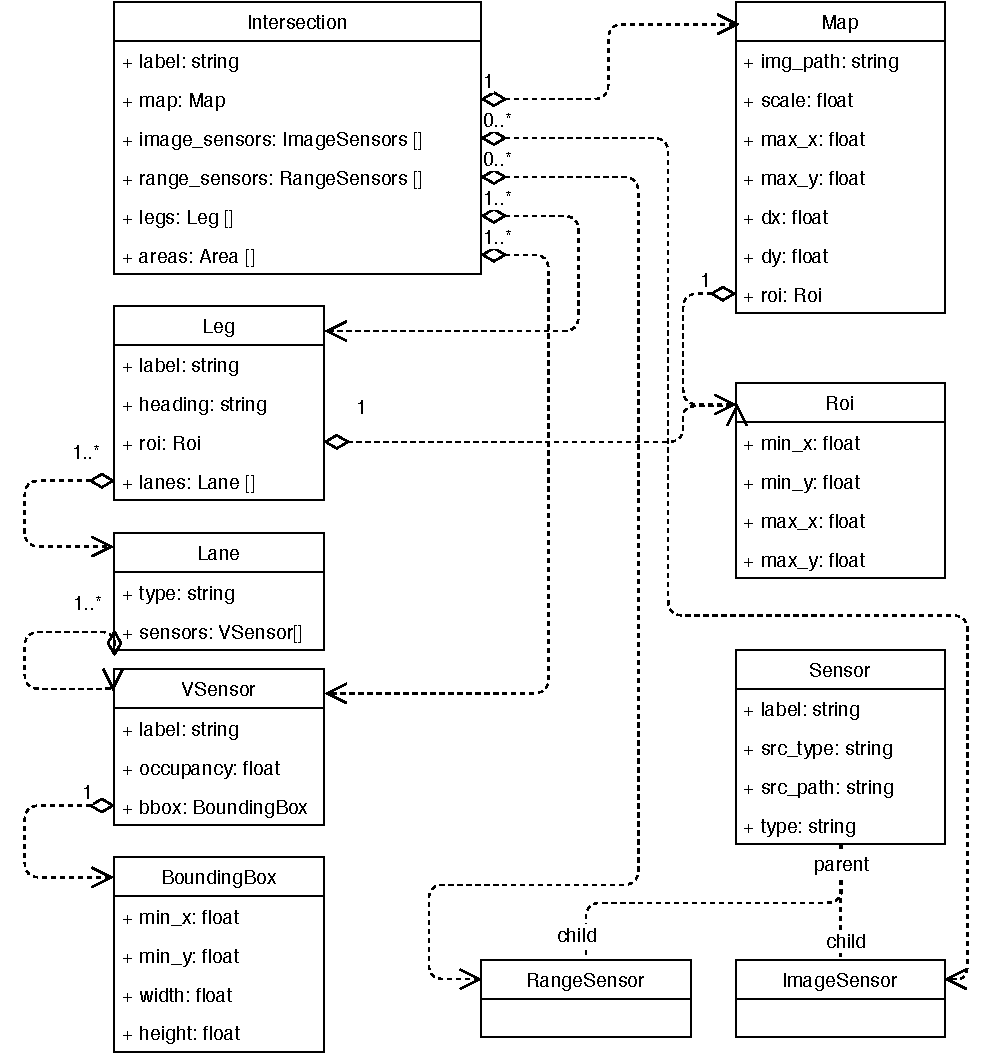
\includegraphics[scale=0.75]{fig/3/data_modelA.pdf}
\caption{UML diagram of defined entities and their relationships}
\label{data_model}
\end{figure}

The purpose of all the labels attributes within each class is to serve as an identifier of the channel in which the entity is publishing or subscribing to; in other words, to identify where data is generated from or where data is going to. For example, channel \texttt{/sensors/range/laser\_1/data/raw} contains raw data from a laser scanner labeled as \texttt{"laser\_1"} and \texttt{/legs/leg\_3/occupancy/} refers to the occupancy level of the leg labeled as \texttt{leg\_3}.

\subsection{Information Structure}

%\todo{Move JSON definition from here!!!}

Data exchanged between processing blocks or any paramater stored in Redis, is formatted using JSON, allowing to use any JSON parser/formatter available in different languages. In addition,  it is possible to create simple scripts to interact with the system. Below are described the two types of data used by the systems: the .imscfg file and the messages and configuration parameters.

\subsubsection{.imscfg file}

For running, the systems requires first a .imscfg file which describes the scenario and the sensors configuration. This information is stored as a JSON object with the properties decribed in table \ref{imscfg_file}.

\begin{table}[ht!]
\footnotesize
\centering
\begin{tabular}{|c | c|}
\hline
\textbf{Property} & \textbf{Description} \\
\hline
name & Name of the configuration \\
\hline
map & Information of the scene, including map, coordinate system \\ 
 & and region of interest. \\
\hline
cameras & List of camera sensors information \\
\hline
range\_sensors & List of range sensors information \\
\hline
legs & List of legs information \\
\hline
intersection & Information of area of the intersection \\
\hline
\end{tabular}
\caption{Properties in .imscfg JSON file}
\label{imscfg_file}
\end{table}

\subsubsection{data messages and configuration parameters}

In addition to .imscfg file, there are different types of messages and parameters which have its own structure, for example used for sensors configuration or processed data. The table \ref{desc_map} gives a description of the types of information used.
% A more detailed documentation is given in appendix TODO.

\begin{table}[ht!]
\footnotesize
\centering
\begin{tabular}{|c | p{8cm}|}
\hline
\textbf{Name} & \textbf{Description} \\
\hline
laser\_pol\_msg & Contains a timestamp, an array of N angles and and array of N measurements \\
\hline
laser\_cart\_msg & Contains a timestamp, an array of N (x, y) coordinates \\
\hline
laser\_cfg & Contains position and orientation information, also has a background model for the laser sensor \\
\hline
occgrid\_msg & Contains a timestamp and an occupancy grid in the form of an MxN array \\
\hline
occgrid\_cfg & Contains occupancy grid configuration for the scene \\
\hline
clusters\_msg & Contains a set of clusters, each of them with an ID and a set of points \\
\hline

clusters\_cfg & Contains configuration about clustering algorithm and parameters \\
\hline

camera\_msg & Frames generated by camera \\
\hline

camera\_cfg & Information and parameters of the camera sensor \\
\hline

blobs\_msg & Bounding boxes detected as objects within a frame from the camera \\
\hline

blobs\_cfg & Parameters used by the image detection process\\
\hline

vs\_occ\_msg & Indicates the occupancy level of a virtual sensor, representing the entrace to or exit from the intersection\\
\hline

vs\_merge\_cfg & Parameters for configuring the merging process of different vs\_occ\_ms messages.\\
\hline

flow\_rate\_msg & Indicates the flow rate entering or exiting the intersection\\
\hline

flow\_cfg & Parameters for estimation of the flow rate, flow status and flow merging configuration\\
\hline

flow\_status\_msg & Indicates the flow status of an entrance or exit at intersection. This is a binary value, with value either "Traffic flowing" or "Traffic stopped".\\
\hline


\end{tabular}
\caption{Description of diferent types of messages and parameters used}
\label{desc_map}
\end{table}

%\todo{Finish table}


\subsection{Processing Blocks} \label{proc_blocks}

As stated in previous section, there are defined four stages in the processing flow, namely, preprocessing, feature analysis, pattern recognition and situation assessment. Within each of these stages there are different methods and techniques used to process the data and it is possible that those methods are suitable to perform fusion between homogeneous or heterogeneous data.

Below are detailed different processing blocks implemented as part of the whole architecture proposal, classified by the stage of processing in which are located in the process flow. Also, it is shown the format of data input, data output and parameters needed for configuration and execution.

Additionaly, there are included some tools and generic blocks used for dataset reading, data visualization and interactive control.

\subsubsection{Preprocessing}
\begin{description}
\item[laser\_background\_remove] \hfill

\begin{figure}[ht!]
\centering
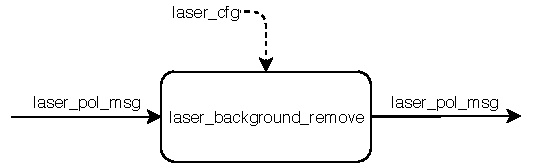
\includegraphics[scale=1]{fig/3/laser_bg_remove.pdf}
\caption{laser\_bg\_remove}
\label{laser_bg_remove}
\end{figure}

This block takes as input a message of type laser\_pol\_msg, which contains raw readings from laser sensor. Also, it takes a laser\_cfg parameter which includes a background model for the laser sensor, generated from a set of scans and taking the maximum measurement in each angle of scanning, defined as follows:

Let suppose we have N scans from the laser and $d_{\theta i}$ be the distance measure at angle $\theta$ in scan $i$. Thus, the background value for that angle $\theta$ is $bg_\theta = max( \{d_{\theta i} | 1 < i < N\})$ and the background model is $bg = \{bg_\theta | \theta \in \Theta\} $ where $\Theta$ is the set of angles of scanning, in this case from -90\degree to 90\degree with 0.5\degree step.

\item[laser\_polar2cart] \hfill

\begin{figure}[ht!]
\centering
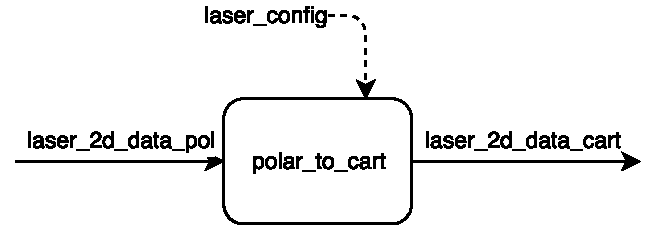
\includegraphics[scale=1]{fig/3/polar2cart.pdf}
\caption{polar\_to\_cartesian}
\label{polar_to_cartesian}
\end{figure}

This block takes as input a message of type laser\_pol\_msg for converting it into cartesian coordinates referenced to global system. For this reason, it also takes a laser\_cfg parameter to include laser position information in the conversion. Output message contains a set of x, y points, referenced to a global coordinate system. This output is obtained from the following equations:

\begin{eqnarray*}
O_x = I_\rho*\cos{\phi}+S_x \\
O_y = I_\rho*\sin{\phi} + S_y \\
\phi = I_\theta + S_\theta
\end{eqnarray*}

Where:

$(S_x, S_y, S_\theta)$: Position and orientation of the laser \\
$(I_\rho, I_\theta )$: Input message (distance and angle arrays) \\
$(O_x, O_y )$: Output message (x and y arrays) \\

\hfill
\item[laser\_cart\_merge] \hfill

\begin{figure}[ht!]
\centering
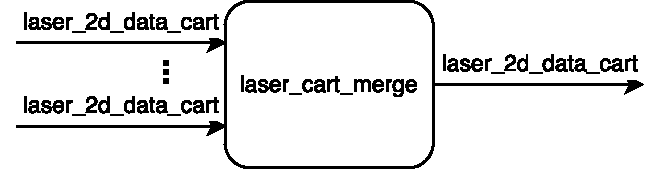
\includegraphics[scale=1]{fig/3/laser_cart_merge.pdf}
\caption{laser\_cart\_merge}
\label{laser_cart_merge}
\end{figure}

This block takes as input messages of type laser\_cart\_msg coming from different sensors and merges them into a single message, based on a sampling period $T$. The objective of this stage is to set a common time-frame and synchronize all the messages to feed to the next blocks.

%\item[camera\_background\_remove] \hfill
%
%\begin{figure}[ht!]
%\centering
%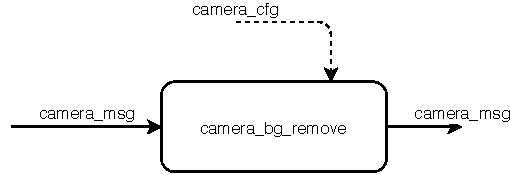
\includegraphics[scale=1]{fig/3/camera_bg_remove.pdf}
%\caption{camera\_background\_remove block}
%\label{cam_bg_remove}
%\end{figure}

\end{description}


\subsubsection{Feature Analysis}
\begin{description}
\item[points\_to\_cluster] \hfill

The input message for this block is a set of points corresponding to objects scanned by lasers. Clustering is performed over this input to identify the points belonging to the same object. The algorithm used in this implementation is DBSCAN, which stands for Density-Based Spatial Clustering of Applications with Noise. This algorithm does not need an estimated number of clusters as input, instead of this, it requires only two parameters: a minimum number of points per cluster, m, and a neighbourhood measure, $\epsilon$. A detailed description of the algorithm, can be found in \cite{Ester96}.

\begin{figure}[ht!]
\centering
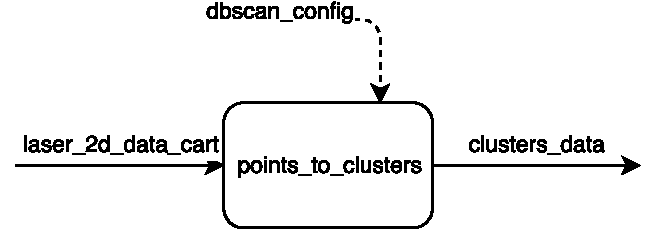
\includegraphics[scale=1]{fig/3/points_to_clusters.pdf}
\caption{points\_to\_clusters}
\label{points_to_clusters}
\end{figure}

The input message for this block is a set of points corresponding to objects scanned by lasers. Clustering is performed over this input to identify the points belonging to the same object. The algorithm used in this implementation is DBSCAN, which stands for Density-Based Spatial Clustering of Applications with Noise. This algorithm does not need an estimated number of clusters as input, instead of this, it requires only two parameters: a minimum number of points per cluster, m, and a neighbourhood measure, $\epsilon$. A detailed description of the algorithm, can be found in \cite{Ester96}.

As output, a message of type clustering\_msg, containing information like clusters ID and set of points belonging to each cluster, is delivered.

\item[points\_to\_occgrid] \hfill

\begin{figure}[ht!]
\centering
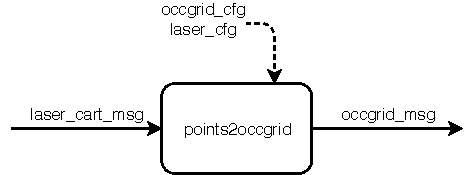
\includegraphics[scale=1]{fig/3/points_to_grid.pdf}
\caption{points\_to\_grid}
\label{points_to_grid}
\end{figure}

This block generates a occupancy grid based on cartesian data from laser sensors. The cartesian data received from sensors is merged in a timeslot basis, filling a buffer for each sensor and processing available data using a defined period $T_{om}$. As parameters, this block receives a cell size for the grid, the laser sensors configuration and the scene configuration. The grid size is of $N_C$ Columns and $N_R$ rows, obtained as follows:

\begin{eqnarray*}
X = x_{max}-x_{min} \\
Y = y_{max}-y_{min} \\
N_C = ceil(X/C)+1 \\
N_R = ceil(Y/C)+1 \\
\end{eqnarray*}

Where $(x_{min}, y_{min})$ and $(x_{max}, y_{max})$ are the bottom-left and top-right coordinates of the region of interest in the scene, respectively.

Each cell of the grid will store a value indicating a probability of that cell being occupied. Initially, all cells have a value of $0.5$. In order, to update the grid using data from laser, the points corresponding to laser position and measures, should be located in a cell of the grid, and then mark it as occupied. The following equations show how a point $P = (P_x, P_y)$ is tranformed to a cell $C_{ij}$, where $i$ is the column and $j$ is the row in the grid:

\begin{eqnarray*}
i = ceil((P_x - x_{min})/C - 0.5) \\
j = N_R - ceil((P_y - y_{min})/C - 0.5) \\
\end{eqnarray*}

Then, the cells that form a straigh line between the cell of laser position and the cells of each laser measure, should be marked as empty. To get the list of these cells Bresenham's algorithm is used. This algorithm is widely used in computer graphics due to it simplicity and because it uses integer arithmetics, making it computationally cheap. The input of this algorithm is a pair of coordinates, the endpoints of the line, and as result, the set of points that completes the line between, is returned.
%\todo{Check bresenham algorithm reference}

As the output, this block generates an occupancy grid of the scene, which is published at a rate defined by the previous period $T_{om}$.
%\todo{update policy}


\item[camera\_blobs] \hfill

\begin{figure}[ht!]
\centering
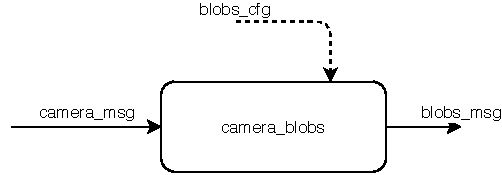
\includegraphics[scale=1]{fig/3/camera_blobs.pdf}
\caption{camera\_blobs}
\label{camera_blobs}
\end{figure}

The purpose of this block is to detect the vehicles from the streaming of video from a camera. To accomplish this task, the YOLOv3 detection system \cite{yolov3} was wraped into a block. The algorithm used by this detector, applies a single neural network to the full image. This network divides the image into regions and predicts bounding boxes and probabilities for each region. These bounding boxes are weighted by the predicted probabilities. The output of this block, are the bounding boxes with high probabilty of being a vehicle.


\item[camera\_blobs2occgrid] \hfill

\begin{figure}[ht!]
\centering
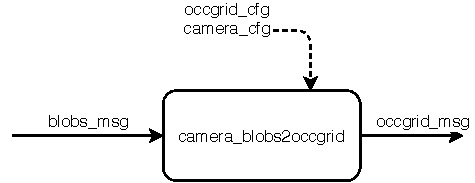
\includegraphics[scale=1]{fig/3/camera_blobs2occgrid.pdf}
\caption{camera\_blobs2occgrid}
\label{camera_blobs2occgrid}
\end{figure}

This block receives bounding boxes corresponding to vehicles and transform them from image coordinate system to the global reference system, Then, it maps the area covered by the boxes into an occupancuy grid in order to mark those cells as occupied in the same fashion as described for the block "points\_to\_occgrid" \ref{points_to_grid}.

\end{description}

\subsubsection{Pattern Recognition}
\begin{description}

\item[virtual\_sensor\_occupancy] \hfill

\begin{figure}[ht!]
\centering
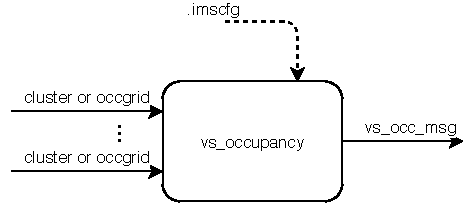
\includegraphics[scale=1]{fig/3/vs_occ.pdf}
\caption{Virtual\_sensor\_occupancy}
\label{vehicle_counter}
\end{figure}

This block accepts different types of inputs, cluster\_msg and occgrid\_msg. It process the incoming data, and generate bounding boxes based on the clusters or based on the occupancy grid, according to the input. Having these bounding boxes, which represent detected vehicles, scene configuration data is loaded and the geometric parameters of the legs and lanes are used to generate virtual sensors at the entry and exit points of the intersection and check the overlaping of detected vehicles with aforemetioned virtual sensors. The output generated by this block is the occupancy percentage of the virtual sensor, represented as a message of type vs\_occ\_msg.
%vehicle counter $v_{cnt}$ is incremented by one when a transition from occupied state to empty state is detected in a new frame.


\hfill

\item[virtual\_sensor\_merge] \hfill
This block is intended to take as inputs different messages of type vs\_occ\_msg and merging them to increase the reliabilty of detection. First, a moving average is calculated over each input to reduce the effect of false positives or false negatives in a single frame. After this, the inputs are merged by a defined method like average, weighted average, maximum or minimum. Then, a new vs\_occ\_msg message is dispatched as output.
\begin{figure}[ht!]
\centering
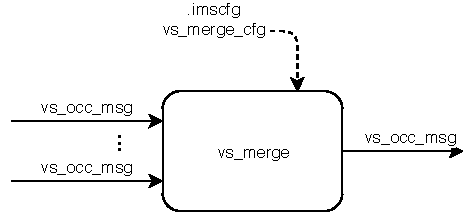
\includegraphics[scale=1]{fig/3/vs_merge.pdf}
\caption{virtual\_sensor\_merge}
\label{virtual_sensor_merge}
\end{figure}



\end{description}


\subsubsection{Situation Assesment}
\begin{description}

\item[virtual\_sensor\_to\_flow\_rate] \hfill

When a message of type vs\_occ\_msg arrives, it is evaluated using a threshold $vo_{th}$, if the occupancy percentage of a virtual sensor is greater than $vo_{th}$, it is considered that there is a vehicle over the sensor in that frame, this is defined as occupied state. This detection is made in a frame basis, thus, a vehicle counter $v_{cnt}$ is incremented by one when a transition from occupied state to empty state is detected in a new frame.

\begin{figure}[ht!]
\centering
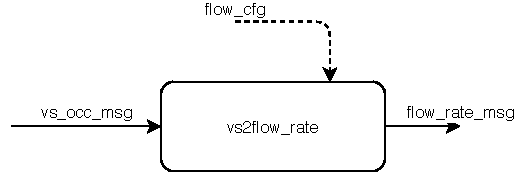
\includegraphics[scale=1]{fig/3/vs2flow.pdf}
\caption{virtual\_sensor\_to\_flow\_rate}
\label{virtual_sensor_to_flow_status}
\end{figure}



Then, a time interval $t_{c}$ is defined for calculating the flow rate $v_{r}$. Defined as the number of transitions during that interval divided by $t_{c}$. The output message type is flow\_rate\_msg.

\hfill

\item[flow\_rate\_to\_flow\_status] \hfill

This block process one or more inputs of type flow\_rate\_msg. If there are more than one input, it merges them using defined policy, like average or maximum. Then, if the flow rate $v_{r}$ is above a flow threshold $f_{th}$, it is considered that the traffic is flowing. Otherwise, traffic is considered stopped.

\begin{figure}[ht!]
\centering
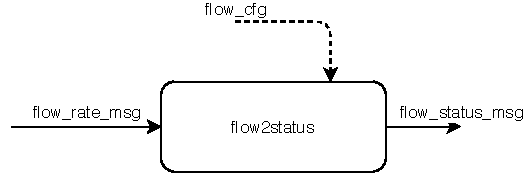
\includegraphics[scale=1]{fig/3/flow2status.pdf}
\caption{flow\_rate\_to\_flow\_status}
\label{flow_rate_to_flow_status}
\end{figure}




\end{description}
%\todo{Check formatting here}
\subsubsection{Tools and Utilities}
\begin{description}

\item[laser\_publisher] \hfill

These blocks are intended to read dataset files containing the information from the sensors and publish this data with the appropriate format and preserving the original rate of the sensors, if needed.

\begin{figure}[ht!]
\centering
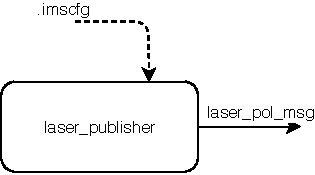
\includegraphics[scale=1]{fig/3/laser_publisher.pdf}
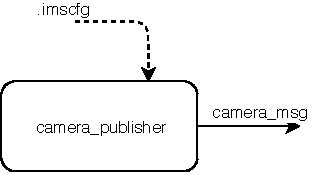
\includegraphics[scale=1]{fig/3/camera_publisher.pdf}
\caption{laser\_publisher and camera\_publisher}
\label{sensors_publishers}
\end{figure}



%\item[camera\_publisher] \hfill
%\begin{figure}[ht!]
%\centering
%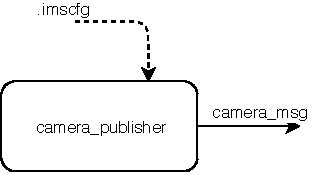
\includegraphics[scale=1]{fig/3/camera_publisher.pdf}
%\caption{camera\_publisher}
%\label{camera_publisher}
%\end{figure}

%\item[dataset\_control] \hfill
%\begin{figure}[ht!]
%\centering
%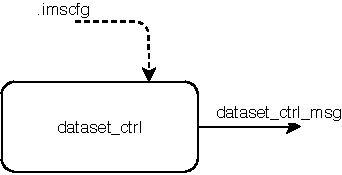
\includegraphics[scale=1]{fig/3/dataset_ctrl.pdf}
%\caption{dataset\_control}
%\label{dataset_control}
%\end{figure}

\item[data\_viewer] \hfill

The objective of this block is to allow the visualisation of the data in any of the processing stages. It has the option to display and XY coordinate system, an occupancy grid or a map of the intersection overlaped with detections or metrics.

\begin{figure}[ht!]
\centering
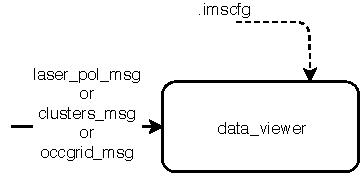
\includegraphics[scale=1]{fig/3/data_viewer.pdf}
\caption{data\_viewer}
\label{data_viewer}
\end{figure}



\end{description}

\section{Conclusions}

A whole intersection management system contains many different components, for example the instrumentation of the junction, the handling of data and information, the control policies and requirements, and the interaction between those elements. None of these items is more relevant than the others and it is for this reason that each one of them should be well conceived having in mind a common framework that allows their scalability, modularity and reliability. When these three features are accomplished, a change or an upgrade of any part of the system will not affect the remaining ones.

It is also important that an Intersection Management System should be flexible, not tied to one deployment or scenario, but also that allows to perform tests over new datasets or junctions, at no extra cost or just with some configuration adjustments. Although it is hard to have a one-rules-them-all system due to the variety of intersections (crossroads with different numbers of legs, roundabouts, T-shaped, Y-shaped, etc.), there are common needs, features and requirements that makes relevant to use an interesection management system looking forward to monitor, control and improve safety and efficiency in transportation.